% !TEX program = xelatex
\documentclass[UTF8,a4paper,12pt]{ctexart}

\usepackage{geometry}
\geometry{left=2.4cm,right=2.4cm,top=2.6cm,bottom=2.6cm}
\usepackage{graphicx}
\usepackage{booktabs}
\usepackage{tabularx}
\usepackage{array}
\usepackage{xcolor}
\usepackage{listings}
\usepackage{hyperref}
\usepackage{url}
\usepackage{float}
\usepackage{subcaption}
\usepackage{amsmath}
\usepackage{fancyhdr}
\usepackage{lastpage}
\usepackage{tikz}
\usetikzlibrary{arrows.meta,positioning,shapes.geometric,fit,calc}

\graphicspath{{fig/}{并行模板/}}
\hypersetup{
  colorlinks=true,
  linkcolor=blue!60!black,
  citecolor=blue!60!black,
  urlcolor=blue!60!black
}

\pagestyle{fancy}
\setlength{\headheight}{15pt}
\fancyhf{}
\lhead{\kaishu 协程技术调研}
\rhead{\kaishu 并行程序设计}
\cfoot{\thepage\ /\ \pageref{LastPage}}

\lstset{
  basicstyle=\ttfamily\small,
  keywordstyle=\color{blue!70!black}\bfseries,
  commentstyle=\color{green!40!black},
  stringstyle=\color{red!60!black},
  numbers=left,
  numberstyle=\tiny\color{gray},
  frame=single,
  breaklines=true,
  showstringspaces=false,
  columns=fullflexible,
  tabsize=2
}

\lstdefinelanguage{Go}{
  morekeywords={package,import,func,var,const,for,go,defer,return,chan,make,select,case,range},
  sensitive=true,
  morecomment=[l]{//},
  morestring=[b]"
}

\lstdefinelanguage{CSharp}{
  morekeywords={async,await,Task,public,class,static,void,int,var,return,new,using},
  sensitive=true,
  morecomment=[l]{//},
  morestring=[b]"
}

\definecolor{diagramBlue}{HTML}{0B4EA2}
\definecolor{diagramTeal}{HTML}{0F8A86}
\definecolor{diagramAmber}{HTML}{C1740B}
\definecolor{diagramSoftBlue}{HTML}{EAF2FB}
\definecolor{diagramSoftTeal}{HTML}{E8F5F3}
\definecolor{diagramSoftAmber}{HTML}{FFF4E3}
\definecolor{diagramLine}{HTML}{9AA9BD}
\tikzset{
  archbox/.style={draw=diagramLine, rounded corners=2pt, thick, align=center, inner sep=6pt, font=\small},
  archblue/.style={archbox, fill=diagramSoftBlue, draw=diagramBlue},
  archteal/.style={archbox, fill=diagramSoftTeal, draw=diagramTeal},
  archamber/.style={archbox, fill=diagramSoftAmber, draw=diagramAmber},
  archarrow/.style={-{Latex[length=2.4mm]}, thick, draw=diagramLine},
  archlabel/.style={font=\footnotesize, text=gray!70!black, align=center}
}

\title{\Huge\bfseries 协程技术调研\\[0.4em]
\Large 从并发演进到底层机制、语言选型与实验验证}
\author{柯云超}
\date{2026 年 6 月}

\begin{document}

\begin{titlepage}
  \centering
  \IfFileExists{并行模板/NKU.png}{
\includegraphics[width=0.72\textwidth]{并行模板/NKU.png}\\[1.2cm]}{}
  {\Large 计算机学院\par}
  \vspace{0.8cm}
  {\huge\bfseries 并行程序设计调研报告\par}
  \vspace{1.2cm}
  {\Huge\bfseries 协程技术调研\par}
  \vspace{0.5cm}
  {\Large 从并发演进到底层机制、语言选型与实验验证\par}
  \vfill
  {\Large 作者：柯云超\par}
  \vspace{0.4cm}
  {\Large 日期：2026 年 6 月\par}
\end{titlepage}

\tableofcontents
\newpage

% ============================================================
\section{摘要}
% ============================================================

随着云服务、网络后端和数据处理系统的并发度不断提高，传统 ``一个请求一个线程'' 的编程方式逐渐遇到内存、调度和可维护性瓶颈。协程提供了一种比操作系统线程更轻量的并发抽象：程序员仍然书写接近同步风格的代码，而编译器和运行时在暂停点保存执行状态，并在 I/O 就绪或调度条件满足时恢复执行。换言之，协程解决的核心问题不是 ``让 CPU 算得更快''，而是 ``让等待变得更便宜''。

本文围绕四个问题展开：并发执行机制为什么会从进程、线程、事件循环演进到协程；有栈协程和无栈协程分别如何保存与恢复执行状态；Go、Java、C++、Python、C\#、Rust 等语言为何选择不同的协程路线；协程在 I/O 密集、CPU 密集和切换开销实验中与线程表现有何差异。本文的实验部分使用 Python、Go、Java 在同一台 Windows/i9-13900H 机器上进行测量：基础微基准覆盖 10K sleep 等待、CPU fib(25) 与调度开销；补充实验加入本地 TCP echo 和 Java virtual thread pinning，用来验证真实 socket 开销和同步锁固定 carrier 线程这两个工程边界。

本文结论可以概括为三点：第一，协程的核心价值是用更低的内存和调度开销承载大规模 I/O 并发，而不是替代并行计算；第二，协程机制需要编译器、语言运行时和操作系统 I/O 多路复用协同完成；第三，语言选型时应关注调度器、取消语义、阻塞调用兼容性、pinning 风险和现有生态，而不是只比较 ``是否支持 async/await''。

\noindent\textbf{关键词：} 协程；有栈协程；无栈协程；异步 I/O；运行时调度；虚拟线程

% ============================================================
\section{引言：协程解决的是等待方式}
% ============================================================

如果把一个网络服务请求拆开看，CPU 真正计算的时间往往只占一小部分，更多时间花在等待数据库、网络、磁盘或远端 RPC 返回。传统线程模型把这种等待表现为内核线程阻塞：每个等待中的请求仍然占用一个线程对象、一个栈空间和调度队列中的位置。事件循环把等待从线程中抽出，但要求程序员手写回调和状态机。协程的出现，正是为了在 ``少量线程承载大量等待'' 和 ``业务代码仍然可读'' 之间取得平衡。

因此，本报告并不把协程理解为某种孤立的语法特性，而是把它看作三层系统共同作用的结果：编译器负责把可暂停函数改写为可恢复状态；运行时负责调度任务、处理定时器和 I/O 就绪事件；操作系统提供非阻塞 I/O 和多路复用接口。只看 `async/await` 关键字，很容易低估运行时和 I/O 子系统的重要性；只看调度器，又会忽略语言层面对错误传播、取消和资源生命周期的影响。

本报告希望达到的目标有三个。第一，用一条清晰的演进线解释协程为何出现；第二，通过有栈/无栈两类实现说明协程底层到底保存了什么；第三，用本机实验和工程选型建议回答 ``什么时候该用协程，什么时候不该用''。

为了避免把报告写成概念罗列，本文将协程放在并发系统的完整链条中分析：上层看它如何改变程序员组织控制流的方式，中层看运行时如何在任务队列、定时器和 I/O 就绪事件之间调度，下层看操作系统线程、非阻塞 I/O 与多路复用接口提供了哪些边界条件。本文的主要贡献可以概括为四点：

\begin{enumerate}
  \item 从 ``等待承载能力'' 而不是 ``语法糖'' 的角度解释协程，区分并发、并行、吞吐量和单请求延迟；
  \item 对比有栈协程与无栈协程在状态保存、调用链透明性、内存占用和函数颜色上的根本差异；
  \item 结合 Go、Java 21、C++20、Python、C\#、Rust 的官方设计或一手资料，说明语言特性、标准库和运行时边界如何共同决定可用性；
  \item 使用 sleep 微基准、本地 TCP echo 和 Java pinning 实验验证协程在等待场景下的优势与边界，并明确实验不能证明 ``协程加速 CPU 计算'' 这一错误结论。
\end{enumerate}

% ============================================================
\section{并发执行机制为何演进到协程}
% ============================================================

\subsection{从进程、线程到事件循环}

早期服务器常用多进程模型，每个请求或连接由独立进程处理。这种方式隔离性强，但进程地址空间、页表、IPC 和上下文切换成本较高。线程共享地址空间，创建与通信成本低于进程，因此成为长期主流。但线程仍由内核抢占式调度，默认栈空间常以 MB 计；当连接数从数千增长到数万甚至百万时，线程模型会同时受到内存占用、调度队列和锁竞争限制。

事件循环模型通过非阻塞 I/O 与 \verb|epoll|、\verb|kqueue|、IOCP 或 \verb|io_uring| 等机制，将大量连接复用到少量线程上\cite{epoll,io_uring}。它解决了线程数量过多的问题，却把程序逻辑拆成大量回调函数：局部变量、异常传播和控制流都被手工搬运到回调链中，形成所谓 ``回调地狱''。协程可以理解为对事件循环的抽象封装：底层仍然等待 I/O 事件，表层却恢复为线性的函数书写方式。

\begin{figure}[H]
  \centering
  \begin{tikzpicture}[node distance=0.85cm]
    \node[archblue, minimum width=2.5cm, minimum height=1.05cm] (proc) {多进程\\\footnotesize 强隔离\\IPC/切换重};
    \node[archblue, minimum width=2.5cm, minimum height=1.05cm, right=of proc] (thread) {多线程\\\footnotesize 共享内存\\栈与锁成本};
    \node[archamber, minimum width=2.7cm, minimum height=1.05cm, right=of thread] (event) {事件循环\\\footnotesize 少量线程\\回调状态机};
    \node[archteal, minimum width=2.5cm, minimum height=1.05cm, right=of event] (coro) {协程\\\footnotesize 用户态挂起\\线性控制流};
    \draw[archarrow] (proc) -- node[archlabel, above]{降低创建成本} (thread);
    \draw[archarrow] (thread) -- node[archlabel, above]{减少阻塞线程} (event);
    \draw[archarrow] (event) -- node[archlabel, above]{隐藏回调状态机} (coro);
    \node[archbox, fill=gray!5, below=0.95cm of $(thread.south)!0.5!(event.south)$, minimum width=8.6cm] (claim)
      {核心问题始终相同：大量正在等待的任务，如何不各自占用昂贵的内核线程？};
    \draw[archarrow, draw=diagramTeal] (claim.north east) .. controls +(1.2,0.9) and +(0,-0.8) .. (coro.south);
  \end{tikzpicture}
  \caption{并发模型从强隔离到轻量等待的演进路径}
  \label{fig:concurrency-evolution}
\end{figure}

\begin{table}[H]
  \centering
  \caption{典型并发模型对比}
  \begin{tabularx}{\textwidth}{lXXXX}
    \toprule
    维度 & 进程 & 线程 & 事件循环 + 回调 & 协程 \\
    \midrule
    调度者 & 操作系统 & 操作系统 & 用户态事件循环 & 用户态调度器/运行时 \\
    切换成本 & 高 & 中 & 低 & 低 \\
    内存成本 & 地址空间和内核结构 & 默认栈较大 & 少量闭包对象 & frame 或小栈 \\
    编程风格 & IPC 明显 & 同步风格 + 锁 & 回调嵌套 & 同步风格 + await/yield \\
    适合场景 & 强隔离任务 & CPU 并行、普通并发 & 底层网络库 & 高并发 I/O、异步业务流 \\
    \bottomrule
  \end{tabularx}
\end{table}

\subsection{协程解决的不是 ``计算速度''，而是 ``等待方式''}

协程的暂停点通常出现在 I/O、定时器、channel 收发或显式 yield 处。暂停时，当前协程让出执行权，运行时调度其他可运行协程；事件就绪后再恢复原协程。这一过程避免了 ``线程阻塞在内核中等待''，也避免了大量线程长期占用栈空间。因此协程最适合高并发 I/O，而不是直接加速 CPU 密集型计算。

更严格地说，协程改善的是系统可同时承载的 \textbf{并发数}，并不自动改善单个任务的 \textbf{计算延迟}。如果一个服务的平均请求耗时大部分由等待组成，那么减少每个等待请求占用的线程资源，就可以在相同硬件上承载更多并发请求；但如果一个任务从头到尾都在消耗 CPU，协程只是多了一层调度抽象，不能减少指令数。JEP 444 在解释虚拟线程时也明确指出，虚拟线程提供的是 scale 而不是 speed：CPU bound 工作不会因为线程数量超过核心数而提高吞吐\cite{jep444}。

这一点也是本文实验设计的分界线：I/O 测试使用 \verb|sleep(0.1s)| 模拟大量等待，目标是观察调度模型能否避免线程排队；CPU 测试使用 \verb|fib(25)|，目标是反证协程并不会改变计算复杂度；切换开销测试只讨论量级，不把不同语言的微基准简单排名。

% ============================================================
\section{协程的定义、分类与底层机制}
% ============================================================

\subsection{定义与心智模型}

协程的概念最早可追溯到 1963 年 Conway 的编译器设计\cite{conway1963design}，1966 年 Bernstein 对其进行了系统化阐述\cite{bernstein1966coroutines}。协程可以被看作 ``可暂停和恢复的函数''。普通函数调用以后必须一路执行到返回，而协程可以在 \verb|await|、\verb|yield| 或阻塞点处挂起，保存局部变量、程序计数位置和必要的运行时信息，之后再由调度器恢复。

\begin{lstlisting}[language=C++,caption={C++20 风格的协程伪代码}]
Task<Response> handle(Request req) {
  auto user = co_await db.query(req.uid);
  auto data = co_await rpc.fetch(user);
  co_return render(data);
}
\end{lstlisting}

上面的代码表面上是顺序执行，实际上每个 \verb|co_await| 都可能把控制权交还给调度器。与回调写法相比，协程把状态机生成工作交给编译器和运行时，降低了业务代码的心智负担。

\subsection{有栈协程与无栈协程}

按是否拥有独立执行栈，协程可以分为有栈协程和无栈协程\cite{moura2009revisiting}。

\begin{itemize}
  \item \textbf{有栈协程}：每个协程拥有自己的用户态栈，切换时保存/恢复寄存器和栈指针。优点是可以在较深调用链中挂起，普通函数和协程函数边界更模糊；缺点是需要管理栈空间和栈增长。Go goroutine 与 Java 21 虚拟线程都接近这一类。
  \item \textbf{无栈协程}：协程函数被编译器改写成状态机，局部变量存放在协程 frame 中。优点是内存更小，编译器优化空间大；缺点是函数颜色问题明显，只有被标记的 async/coroutine 函数才能挂起。C++20、Python asyncio、C\# async/await、Rust async 都属于这一类。
\end{itemize}

\begin{table}[H]
  \centering
  \caption{有栈协程与无栈协程的工程差异}
  \begin{tabularx}{\textwidth}{lXX}
    \toprule
    维度 & 有栈协程 & 无栈协程 \\
    \midrule
    状态保存 & 独立用户态栈，保存栈指针和寄存器 & 编译器生成 frame，保存局部变量和状态号 \\
    挂起位置 & 可在较深调用链中挂起 & 通常只能在 async/coroutine 函数中挂起 \\
    对旧代码影响 & 更接近透明迁移，函数颜色问题弱 & 同步/异步 API 分裂明显，函数颜色问题强 \\
    单任务内存 & KB 级起步，依赖栈增长策略 & 字节到数百字节级，依赖 frame 大小 \\
    典型代表 & Go goroutine、Java 21 virtual thread & C++20、Python asyncio、C\#、Rust async \\
    主要风险 & 栈管理、pinning、运行时调度复杂 & 生命周期、取消传播、阻塞调用毒化事件循环 \\
    \bottomrule
  \end{tabularx}
  \label{tab:stackful-stackless}
\end{table}

\subsection{无栈协程：编译器生成状态机}

无栈协程的典型实现是编译器把函数拆成多个状态。每个挂起点对应一个状态编号，局部变量和临时值存放在 frame 中，恢复时根据状态跳转到对应位置继续执行。C\# 编译器生成 \verb|IAsyncStateMachine|，C++20 编译器生成 coroutine frame 和 \verb|coroutine_handle|，Python 的 \verb|async def| 返回 coroutine 对象，运行时将其包装为 Task 后由事件循环推进\cite{pep492}。

这种方式的优势是内存占用可控，很多协程 frame 只有几十到几百字节；切换本质上接近一次函数调用或间接跳转。但它也带来函数颜色问题：普通函数不能直接 \verb|await|，同步 API 与异步 API 需要分别维护。

\begin{figure}[H]
  \centering
  \begin{tikzpicture}[node distance=0.95cm]
    \node[archblue, minimum width=2.25cm, minimum height=0.95cm] (src)
      {源码\\\footnotesize async/co\_await};
    \node[archamber, minimum width=2.45cm, minimum height=0.95cm, right=of src] (rewrite)
      {编译器改写\\\footnotesize 拆分挂起点};
    \node[archteal, minimum width=2.55cm, minimum height=0.95cm, right=of rewrite] (frame)
      {Coroutine Frame\\\footnotesize 状态号 + 局部变量};
    \node[archblue, minimum width=2.45cm, minimum height=0.95cm, right=of frame] (resume)
      {resume()\\\footnotesize 跳回状态 N};

    \draw[archarrow] (src) -- node[archlabel, above]{生成} (rewrite);
    \draw[archarrow] (rewrite) -- node[archlabel, above]{保存} (frame);
    \draw[archarrow] (frame) -- node[archlabel, above]{恢复} (resume);

    \node[archbox, fill=gray!5, below=0.75cm of frame, minimum width=9.4cm] (states)
      {状态机视角：S0 发起 I/O $\rightarrow$ S1 等待就绪 $\rightarrow$ S2 读取结果 $\rightarrow$ S3 返回};
    \draw[archarrow, draw=diagramTeal] (states.north west) .. controls +(-0.7,0.6) and +(0,-0.7) .. (frame.south);
  \end{tikzpicture}
  \caption{无栈协程的核心：编译器把线性函数改写为带 frame 的状态机}
  \label{fig:stackless-state-machine}
\end{figure}

C++20 的设计最能体现无栈协程的 ``低层机制'' 特征。标准语言并不规定 \verb|Task|、事件循环或 I/O 后端，而是定义一套可组合协议：协程函数通过 \verb|promise_type| 决定返回对象、初始/最终挂起策略和异常传递；\verb|co_await| 表达式通过 \verb|await_ready|、\verb|await_suspend|、\verb|await_resume| 三个方法决定是否立即完成、挂起后把控制权交给谁、恢复后返回什么值；\verb|coroutine_handle| 则是运行时恢复或销毁 frame 的句柄\cite{cppreferenceCoroutines}。因此，C++20 coroutine 本身更像 ``可暂停函数的 ABI''，而不是完整并发框架。

这一设计带来两个工程后果。第一，C++ 项目必须自己选择 executor、事件循环和取消模型：同样是 \verb|co_await socket.read()|，背后可以是 epoll、IOCP、io\_uring 或线程池。第二，frame 生命周期非常关键：如果 awaiter 在 I/O 未完成时销毁了 frame，或恢复已经完成/取消的 frame，就会造成悬空句柄和未定义行为。相比之下，Python、C\#、Rust 的 async 运行时在任务对象层面封装了更多生命周期管理，但本质上仍然是在推进类似的状态机。

\subsection{有栈协程：用户态上下文切换}

有栈协程的切换通常包括保存 callee-saved 寄存器、保存旧栈指针、切换到新栈并恢复寄存器。简化后的 x86\_64 上下文切换可以概括为如下形式：

\begin{lstlisting}[language={[x86masm]Assembler},caption={有栈协程上下文切换示意}]
switch_ctx:
    push   rbp
    push   rbx
    push   r12-r15
    mov    [rdi], rsp    ; 保存旧栈指针
    mov    rsp, [rsi]    ; 切换到新协程栈
    pop    r15-r12
    pop    rbx
    pop    rbp
    ret
\end{lstlisting}

Go 的 goroutine 初始栈很小（2KB），并可按需增长到 GB 级；运行时通过 G-M-P 调度模型把大量 goroutine 映射到较少的操作系统线程上。Java 21 虚拟线程则把轻量线程引入 JVM 标准能力，虚拟线程运行在 carrier 平台线程之上，由 JVM 调度并在多数 JDK 阻塞 I/O 处自动让出 carrier\cite{jep444}。

有栈协程的关键不是 ``每个任务都有一个完整线程''，而是 ``每个任务拥有可保存的调用栈，而这些栈不必一一绑定内核线程''。Go 在早期经历过分段栈和连续栈策略的演进，现代 goroutine 使用可增长栈：运行时在函数调用前检查栈空间，不足时复制到更大的栈并更新指针。这样既保留了普通函数调用链可以挂起的优势，又避免了 OS 线程默认大栈带来的巨大浪费。Java 虚拟线程也采取类似思路：虚拟线程的栈帧可以在挂起时从 carrier 平台线程栈上卸载，之后再装载恢复。

不过，有栈协程的透明性也有代价。运行时必须知道哪些阻塞点可以安全卸载，哪些阻塞点会把任务固定在 carrier 上。JEP 444 特别指出，Java 虚拟线程在进入 \verb|synchronized| 代码块或执行某些 native/foreign 调用时可能发生 pinning：虚拟线程被固定在 carrier 线程上，阻塞期间 carrier 不能服务其他虚拟线程\cite{jep444}。Go 也存在类似边界：系统调用、cgo、长时间 CPU 循环都会影响调度器复用 M 的能力，因此 Go runtime 需要 sysmon、netpoller 和抢占机制共同维持公平性。

\subsection{术语边界：协程、线程、Future 与 Fiber}

协程相关术语常被混用，调研时需要先划清边界。本文使用如下约定：

\begin{itemize}
  \item \textbf{Coroutine} 强调可暂停/恢复的控制流抽象，可以是有栈，也可以是无栈。
  \item \textbf{Fiber / virtual thread / goroutine} 通常强调由运行时调度的轻量执行单元，更接近有栈协程或轻量线程。
  \item \textbf{Future / Promise / Task} 通常表示一个异步结果或被调度的协程实例。Future 不一定正在运行；它可以是惰性的，也可以被 executor 轮询或调度。
  \item \textbf{Async I/O} 是 I/O 后端能力，不等于协程。没有 async/await 也可以用回调或事件循环做异步 I/O；协程只是把异步 I/O 包装为更线性的控制流。
\end{itemize}

以 Rust 为例，\verb|async fn| 返回的 Future 默认是惰性的，只有被 executor poll 时才向前推进\cite{rustAsyncBook}；以 C\# 为例，\verb|async| 方法通常返回热任务，调用后就开始执行到第一个未完成的 await\cite{dotnetAsync}。二者表面语法相似，但调度时机、取消传播和资源生命周期不同。这说明 ``支持 async/await'' 并不是充分信息，必须进一步追问运行时模型。

% ============================================================
\section{主流语言支持对比}
% ============================================================

\subsection{有栈协程语言：Go 与 Java 21}

Go 语言自 1.0（2012）起就内建了 goroutine 和 channel。goroutine 是有栈协程，初始栈仅 2KB，运行时通过 G-M-P 模型调度\cite{goScheduler}：G 是 goroutine，M 是操作系统线程，P 是逻辑处理器（持有本地运行队列）。网络 I/O 通过内建的 netpoller（底层使用 epoll/kqueue/IOCP）自动挂起和恢复。Go 1.14 引入基于信号的抢占式调度，避免长时间计算的 goroutine 饿死其他任务\cite{goRuntime}。

\begin{figure}[H]
  \centering
  \begin{tikzpicture}[node distance=0.75cm]
    \node[archamber, minimum width=1.45cm, minimum height=0.8cm] (m1) {M\\\footnotesize OS 线程};
    \node[archamber, minimum width=1.45cm, minimum height=0.8cm, below=0.7cm of m1] (m2) {M\\\footnotesize OS 线程};
    \node[archblue, minimum width=1.55cm, minimum height=0.8cm, right=1.35cm of m1] (p1) {P\\\footnotesize 逻辑处理器};
    \node[archblue, minimum width=1.55cm, minimum height=0.8cm, right=1.35cm of m2] (p2) {P\\\footnotesize 逻辑处理器};
    \node[archteal, minimum width=1.0cm, minimum height=0.68cm, right=1.15cm of p1] (g1) {G};
    \node[archteal, minimum width=1.0cm, minimum height=0.68cm, right=0.45cm of g1] (g2) {G};
    \node[archteal, minimum width=1.0cm, minimum height=0.68cm, right=1.15cm of p2] (g3) {G};
    \node[archbox, fill=gray!5, minimum width=2.4cm, minimum height=0.75cm, right=1.0cm of g2] (netpoll)
      {netpoller\\\footnotesize I/O 就绪队列};

    \draw[archarrow] (m1) -- node[archlabel, above]{绑定} (p1);
    \draw[archarrow] (m2) -- (p2);
    \draw[archarrow] (p1) -- node[archlabel, above]{调度} (g1);
    \draw[archarrow] (p1) -- (g2);
    \draw[archarrow] (p2) -- (g3);
    \draw[archarrow, draw=diagramTeal] (netpoll.west) -- node[archlabel, above]{恢复 G} (g2.east);
    \draw[archarrow, dashed] (p2.north east) .. controls +(0.8,0.9) and +(-0.8,-0.9) .. node[archlabel, right]{work stealing} (p1.south east);
  \end{tikzpicture}
  \caption{Go GMP 调度模型：大量 goroutine 复用少量操作系统线程}
  \label{fig:go-gmp}
\end{figure}

Java 21（2023）通过 JEP 444 引入虚拟线程\cite{jep444}。虚拟线程是 JVM 管理的有栈协程，运行在少量 carrier 平台线程之上。JDK 内所有阻塞 API（Socket、JDBC、\verb|Thread.sleep|）已被改造为在阻塞点自动 yield carrier，而非阻塞内核线程。虚拟线程的最大卖点是 ``同步代码无需修改''：开发者用 \verb|Thread.ofVirtual()| 替换 \verb|new Thread()| 即可获得协程级并发能力。但 \verb|synchronized| 块和 JNI 调用会把虚拟线程 pin 到 carrier 上，是使用时的主要陷阱。

Go 与 Java 21 的共同点是把复杂度更多放入运行时和标准库：开发者仍然可以写阻塞式代码，运行时在网络 I/O、sleep、park 等可识别阻塞点把执行权交还给调度器。差异在于，Go 从语言诞生起就围绕 goroutine/channel 设计，标准库 I/O、GC 和调度器天然协同；Java 21 则是在已有 JVM、线程 API 和海量同步生态之上引入虚拟线程，因此最重要的价值是兼容迁移。换句话说，Go 更像 ``并发原生语言''，Java 虚拟线程更像 ``为旧同步生态补上一层轻量线程能力''。

从深入调研角度看，这两种有栈路线真正要比较的不是 ``谁创建任务更快''，而是阻塞点覆盖范围、调度公平性和诊断工具。Go 的 goroutine dump、race detector、pprof 等工具围绕 goroutine 构建；Java 的虚拟线程则继续复用线程 dump、JFR 和现有调试生态。这说明协程机制能否落地，和可观测性同样相关。

\subsection{无栈协程语言：C++20、Python、C\#、Rust}

C++20（2020）在语言层面引入了 \verb|co_await|、\verb|co_yield|、\verb|co_return| 三个关键字，但标准库不提供调度器、Task 类型或异步 I/O。开发者需要依赖 cppcoro、libcoro 或 Boost.Asio 等第三方库来构建完整的异步生态。这种 ``只给机制，不给策略'' 的设计给予了最大灵活性，但也提高了入门门槛。

Python 的 asyncio（PEP 492/525/530）\cite{pep492} 使用单线程事件循环，\verb|async def| 返回 coroutine 对象，被包装为 Task 后由事件循环推进。底层通过 \verb|selector| 模块调用 epoll/kqueue 等系统调用。Python 的 GIL 限制了 CPU 密集型任务的并行能力，因此 asyncio 最适合 I/O 密集型场景。阻塞同步调用（如 \verb|time.sleep|、\verb|requests.get|）会阻塞整个事件循环，是使用时的主要风险。

C\# 5.0（2012）是现代 async/await 的 ``开山鼻祖''。编译器把 \verb|async| 方法改写为 \verb|IAsyncStateMachine|，\verb|Task| 类型充当 Future，\verb|SynchronizationContext| 决定恢复在哪个线程（WinForms/WPF 回 UI 线程，ASP.NET 回请求线程）。C++20、Rust、Python 的 async/await 在语义和实现上都深度借鉴了 C\# 的设计。

Rust（1.39，2019）的 \verb|async/await| 编译为 \verb|Future| 状态机，但语言不提供运行时，需要 tokio 或 async-std 等第三方库。Rust 的所有权和生命周期系统使得 async 函数的 frame 管理更复杂，学习曲线较陡，但换来了零成本抽象和无垃圾回收的性能保证。

无栈路线的共同点是 ``显式标记可暂停边界''。这使编译器能精确知道哪些局部变量跨越 await 点，需要被提升到 frame；也使程序员必须在 API 设计上区分同步函数与异步函数。其优势是内存占用和控制力，劣势是函数颜色、生命周期和取消传播更显性。Python 与 C\# 通过标准库和语言运行时把 Task 模型封装得较完整；Rust 和 C++ 则把更多策略留给生态，换取系统级控制能力。这也是为什么同样是 async/await，Web 爬虫、桌面 UI、嵌入式服务和高性能网络库的最佳语言选择会不同。

\begin{table}[H]
  \centering
  \caption{主流语言协程能力对比}
  \begin{tabularx}{\textwidth}{lXXXX}
    \toprule
    语言 & 关键机制 & 类型 & 调度器 & 主要特点 \\
    \midrule
    Go & \texttt{go}/channel & 有栈 & GMP 内建 & 语法轻，普通函数可直接作为 goroutine \\
    Java 21 & Virtual Thread & 有栈 & JVM ForkJoin & 保持同步代码风格，降低迁移成本 \\
    C++20 & \texttt{co\_await} & 无栈 & 标准不提供 & 只给底层机制，Task 和 I/O 需库实现 \\
    Python & \texttt{async/await} & 无栈 & 单线程事件循环 & 适合 I/O；CPU 密集受 GIL 限制 \\
    C\# & \texttt{async/await} & 无栈 & 线程池/上下文 & 工程化成熟，UI/服务端生态完善 \\
    Rust & \texttt{async/await} & 无栈 & 第三方运行时 & 零成本抽象强，但生态和学习成本高 \\
    \bottomrule
  \end{tabularx}
\end{table}

\begin{table}[H]
  \centering
  \caption{不同语言协程设计背后的关键取舍}
  \begin{tabularx}{\textwidth}{lXXX}
    \toprule
    语言路线 & 运行时承担 & 程序员承担 & 适合的组织形态 \\
    \midrule
    Go goroutine & 调度、网络轮询、栈增长、抢占 & 避免 goroutine 泄漏，设计 channel/ctx 取消 & 新建网络服务、微服务、并发原生代码 \\
    Java virtual thread & carrier 调度、JDK 阻塞 API 改造、线程诊断复用 & 避免 pinning，控制同步锁和 native 调用 & JVM 旧系统迁移、同步代码高并发化 \\
    Python asyncio & 事件循环、Task、selector、TaskGroup & 不阻塞 loop，显式 await，处理取消 & I/O 脚本、Web、爬虫、轻量后端 \\
    C\# async/await & Task、线程池、同步上下文、异常包装 & 避免 sync-over-async 和上下文死锁 & UI、服务端、企业应用 \\
    Rust/C++ async & 低层状态机和零成本抽象 & 选择 executor/I/O 后端，管理生命周期与取消 & 系统级网络、低延迟服务、库开发 \\
    \bottomrule
  \end{tabularx}
  \label{tab:language-tradeoff}
\end{table}

\subsection{运行时与操作系统的协同}

协程不是脱离操作系统独立存在的机制。它通常需要三层协作：

\begin{enumerate}
  \item \textbf{编译器或解释器}：识别 async/await、yield 或 coroutine 关键字，生成 frame、状态机和恢复入口。
  \item \textbf{语言运行时}：维护可运行队列、挂起队列、Task/Future、定时器和调度策略；Go 还包括 work stealing、netpoller 和抢占逻辑\cite{goRuntime}。
  \item \textbf{操作系统}：提供非阻塞 I/O、多路复用、线程和定时器等基础能力。运行时等待 fd 就绪后，再恢复对应协程。
\end{enumerate}

\begin{figure}[H]
  \centering
  \begin{tikzpicture}[node distance=0.85cm]
    \node[archblue, minimum width=3.25cm, minimum height=1.0cm] (compiler)
      {编译器/解释器\\\footnotesize frame、状态机、恢复入口};
    \node[archteal, minimum width=3.25cm, minimum height=1.0cm, right=of compiler] (runtime)
      {语言运行时\\\footnotesize 队列、Task/Future、定时器};
    \node[archamber, minimum width=3.25cm, minimum height=1.0cm, right=of runtime] (os)
      {操作系统\\\footnotesize 非阻塞 I/O、多路复用、线程};

    \draw[archarrow] (compiler) -- node[archlabel, above]{挂起/恢复协议} (runtime);
    \draw[archarrow] (runtime) -- node[archlabel, above]{注册 fd/定时器} (os);
    \draw[archarrow, bend left=20, draw=diagramTeal] (os.south) to node[archlabel, below]{就绪通知} (runtime.south);
    \draw[archarrow, draw=diagramTeal] (runtime.north) .. controls +(-0.4,0.75) and +(0.4,0.75) ..
      node[archlabel, above, pos=0.52, fill=white, inner sep=1pt]{恢复协程} (compiler.north);

    \node[archbox, fill=gray!5, below=0.75cm of runtime, minimum width=8.8cm] (boundary)
      {协程切换可以在用户态完成，但 I/O 就绪、CPU 时间和内存回收仍受 OS/运行时约束。};
  \end{tikzpicture}
  \caption{协程机制的三层协同：语法、运行时与操作系统能力共同闭环}
  \label{fig:three-layer-runtime}
\end{figure}

这三层之间的边界决定了协程的实际可用性。例如 C++20 语言标准只定义协程语义和编译器改写规则，不规定调度器与 I/O 模型；因此 C++ 项目必须选择或实现自己的 Task、executor 和 I/O 后端。Python asyncio 则把运行时收敛到单线程事件循环，降低了模型复杂度，但同步阻塞调用会直接阻塞整个 loop。Go 和 Java 21 的路线更接近 ``运行时替程序员接管阻塞点''，因此迁移体验更好，但需要运行时和标准库对阻塞 API 做更深改造。

这里还存在一个容易混淆的问题：协程调度器并不能绕过操作系统。即使协程切换发生在用户态，最终 I/O 仍然依赖 fd 就绪通知、完成端口或内核异步 I/O；CPU 时间仍然由 OS 线程获得；内存回收仍然受 GC 或 allocator 影响。所谓 ``百万协程'' 的可行性，前提是绝大多数协程处于等待态且 frame/栈足够小，而不是百万个任务同时消耗 CPU。报告中的选型建议因此不把协程视为独立银弹，而把它看作语言运行时对 OS 能力的一层组织方式。

\subsection{错误、取消与结构化并发}

协程系统真正进入工程实践后，最容易被忽略的不是创建任务，而是任务失败、取消和退出时的资源管理。手工创建大量协程而不等待其结束，会造成所谓协程泄漏：任务继续运行但调用方已经失去引用，异常无法传播，资源也无法及时释放。结构化并发的核心思想是让父任务拥有子任务的生命周期：父任务退出前必须等待或取消子任务，错误沿着明确的作用域传播。

不同语言对这一问题的支持程度不同。Python 3.11 引入的 \verb|asyncio.TaskGroup| 能够把一组任务绑定到同一个作用域；Go 生态中常用 \verb|errgroup| 管理 goroutine 的错误传播和取消；Kotlin、Swift、Trio 等系统也把结构化并发作为核心设计。虽然这些机制不总是被称为 ``协程机制''，但它们决定了协程代码能否在真实系统中长期维护。对于课程报告中的选型建议而言，``有没有协程'' 只是第一层问题，``协程失败后谁负责收尾'' 才是工程上更关键的问题。

取消语义尤其值得单独强调。协程被取消时，运行时通常只能在下一个挂起点注入取消信号；如果任务长期执行 CPU 循环、持有锁或调用不可中断的同步 API，取消就会延迟甚至失效。Python 文档把 TaskGroup 作为更安全的并发组织方式，是因为它能在子任务失败时取消同组任务并聚合异常\cite{pythonTaskGroup}。C\# 中常用 \verb|CancellationToken| 显式传递取消；Go 中常用 \verb|context.Context|；Rust/tokio 中取消往往通过 drop future 或 select 分支体现。不同语言的取消机制不同，但共同目标都是防止 ``任务已经失败，其他协程还在后台继续跑''。

% ============================================================
\section{实验设计与结果}
% ============================================================

\subsection{实验环境与方法}

实验在同一台本机上运行，硬件与软件环境如下：

\begin{itemize}
  \item CPU：13th Gen Intel(R) Core(TM) i9-13900H，14 核 20 逻辑处理器；
  \item 操作系统：Windows 11 Home China 64-bit，版本 10.0.26200；
  \item Python：3.12.9；Go：1.25.6；Java：OpenJDK 21.0.5；
  \item 基础微基准日期：2026 年 5 月 27 日；补充 TCP 与 pinning 边界实验日期：2026 年 6 月 5 日。
\end{itemize}

测试分为五类：I/O 密集型测试创建 10000 个任务，每个任务 sleep 100 ms，用于隔离大量等待任务的承载能力；CPU 密集型测试创建 1000 个任务，每个任务计算 \verb|fib(25)|，用于反证 ``协程不自动加速计算''；上下文切换测试使用大量 yield/sleep(0)、channel 交互或轻量任务估计调度开销；本地 TCP echo 测试创建 1000 次 loopback 连接，纳入真实 socket connect/write/read/close 开销；Java pinning 测试在虚拟线程中对比普通 sleep 与 \verb|synchronized| 内 sleep，用来验证同步锁对 carrier 线程的固定效应。基础微基准重复 5 次，TCP echo 重复 5 次，pinning 实验重复 3 次，均报告均值和标准差。

\subsection{I/O 密集型结果}

\begin{figure}[H]
  \centering
  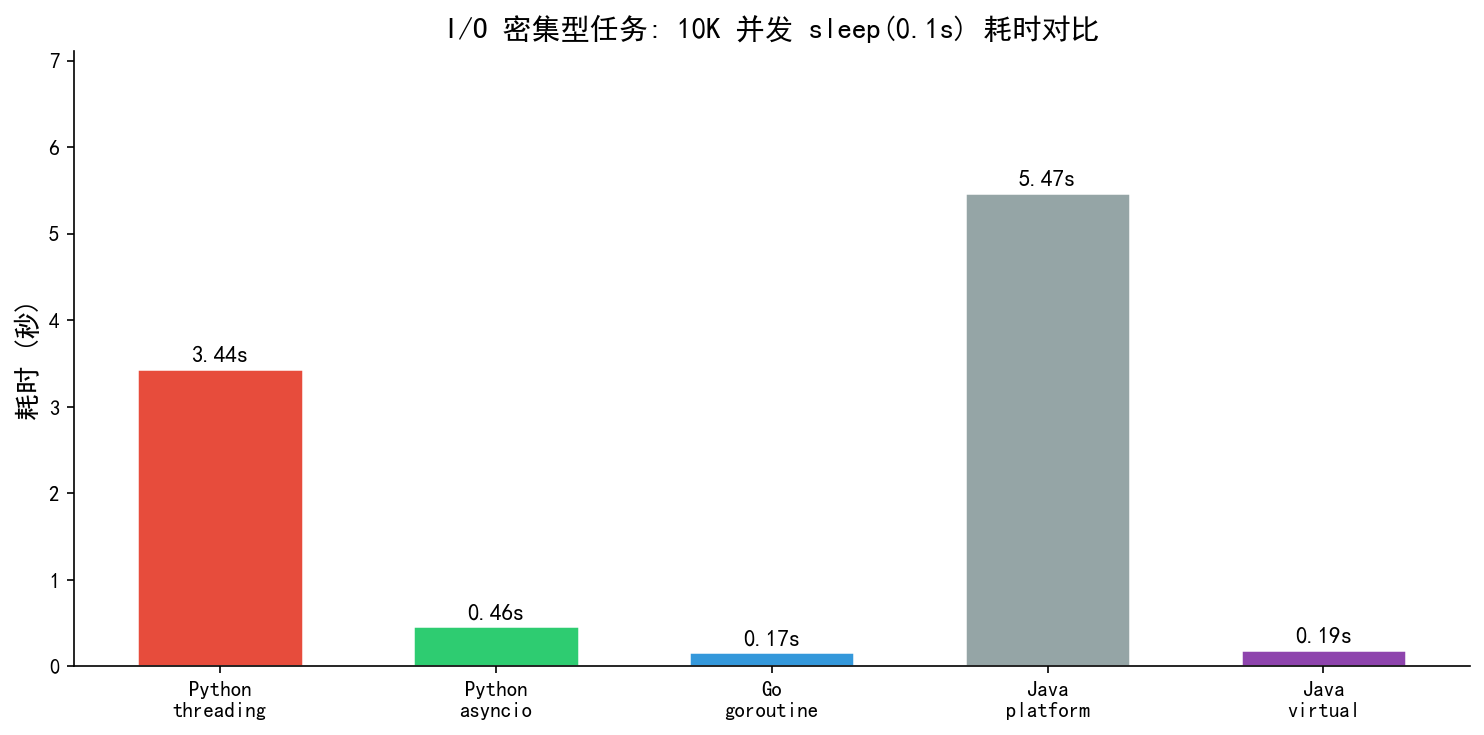
\includegraphics[width=0.88\textwidth]{io_throughput.png}
  \caption{10000 个 I/O 等待任务耗时对比（5 次重复，误差线为标准差）}
  \label{fig:io}
\end{figure}

\begin{table}[H]
  \centering
  \caption{I/O 密集型实验结果（5 次重复）}
  \begin{tabularx}{\textwidth}{l l X}
    \toprule
    模型 & 10000 任务耗时 & 对照口径 \\
    \midrule
    Python threading & 3.130$\pm$0.426 s & Python 线程基线 \\
    Python asyncio & 0.446$\pm$0.012 s & 比 Python threading 快约 7.0$\times$ \\
    Go goroutine & 0.116$\pm$0.020 s & Go 运行时内建轻量任务 \\
    Java platform thread（200 固定线程池） & 5.458$\pm$0.013 s & Java 线程池基线 \\
    Java virtual thread & 0.235$\pm$0.173 s & 比 Java platform thread 快约 23.2$\times$ \\
    \bottomrule
  \end{tabularx}
\end{table}

结果符合预期：I/O 密集场景中，协程/虚拟线程能在等待期间释放执行权，使少量内核线程服务大量逻辑任务。Python asyncio 相比 Python threading 快约 7.0 倍；Go goroutine 和 Java 虚拟线程都能在 0.2 秒量级完成 10000 个 sleep 任务，Java 虚拟线程相比固定平台线程池快约 23.2 倍。Java 虚拟线程的标准差较大（$\pm$173 ms），可能与 JIT 预热有关。

需要强调的是，这里观察到的加速并不是 ``sleep 被算得更快''，而是调度模型避免了大量 OS 线程同时阻塞。平台线程池只能让固定数量的线程并发等待，剩余任务排队；协程和虚拟线程则可以把等待任务挂起，让底层少量线程继续推进其他就绪任务。因此，I/O 密集实验本质上测量的是等待任务的承载能力，而不是计算吞吐能力。

\subsection{本地 TCP echo：加入真实 socket 开销}

仅使用 sleep 模拟等待有一个明显缺陷：它能隔离调度器差异，却没有覆盖 socket 连接建立、读写、关闭和操作系统协议栈开销。为了让实验更接近网络服务，本文补充了本地 TCP echo 测试：在 loopback 地址上启动 echo server，客户端发起 1000 次连接，每次发送固定长度 payload，读取回显后关闭连接。为了降低 Windows loopback 与连接积压造成的瞬时失败，客户端按批次发起连接；每组重复 5 次，结果如表 \ref{tab:tcp-echo} 所示。

\begin{table}[H]
  \centering
  \caption{本地 TCP echo 实验结果（1000 次连接，5 次重复）}
  \begin{tabularx}{\textwidth}{l l X}
    \toprule
    模型 & 总耗时 & 解释 \\
    \midrule
    Python asyncio & 1.632$\pm$1.119 s & 单事件循环管理连接生命周期 \\
    Python threading & 1.948$\pm$0.303 s & 批量创建线程执行阻塞 socket 调用 \\
    \bottomrule
  \end{tabularx}
  \label{tab:tcp-echo}
\end{table}

这个结果比 sleep 微基准更保守：asyncio 只比 threading 快约 1.2 倍，而且标准差较大。原因是该测试中的主要开销不再只是 ``等待 100 ms''，还包括 TCP 三次握手、内核缓冲区、连接关闭、server 端调度以及 Windows loopback 的抖动。换言之，当真实协议栈和连接管理成本进入实验，协程的优势会被稀释；但 asyncio 仍略快，说明在连接生命周期由事件循环统一管理时，减少线程创建和阻塞调度仍然有收益。更重要的是，这个实验提醒我们不能只拿 sleep 微基准宣称 ``协程一定快很多''，真实服务还要继续考虑连接池、HTTP/TLS、序列化、数据库驱动和背压策略。

\subsection{CPU 密集型与切换开销}

\begin{figure}[H]
  \centering
  \begin{subfigure}{0.48\textwidth}
    \centering
    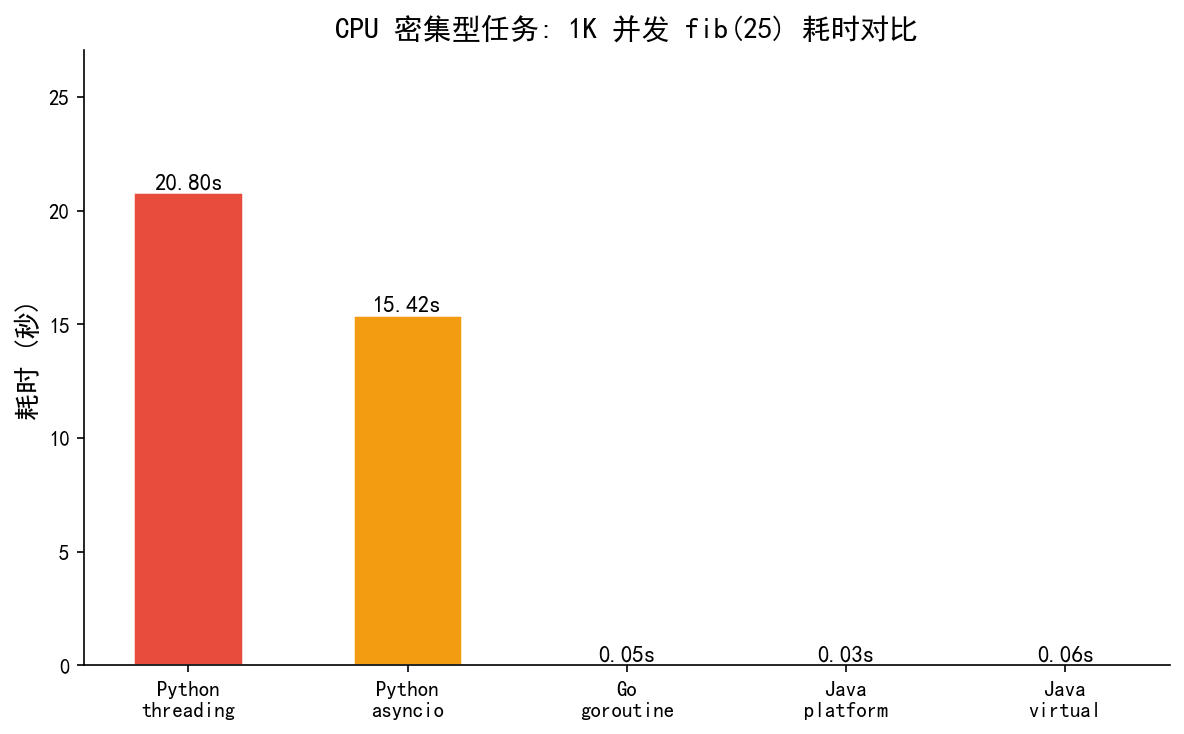
\includegraphics[width=\linewidth]{cpu_benchmark.png}
    \caption{CPU 密集型 fib(25)}
  \end{subfigure}
  \hfill
  \begin{subfigure}{0.48\textwidth}
    \centering
    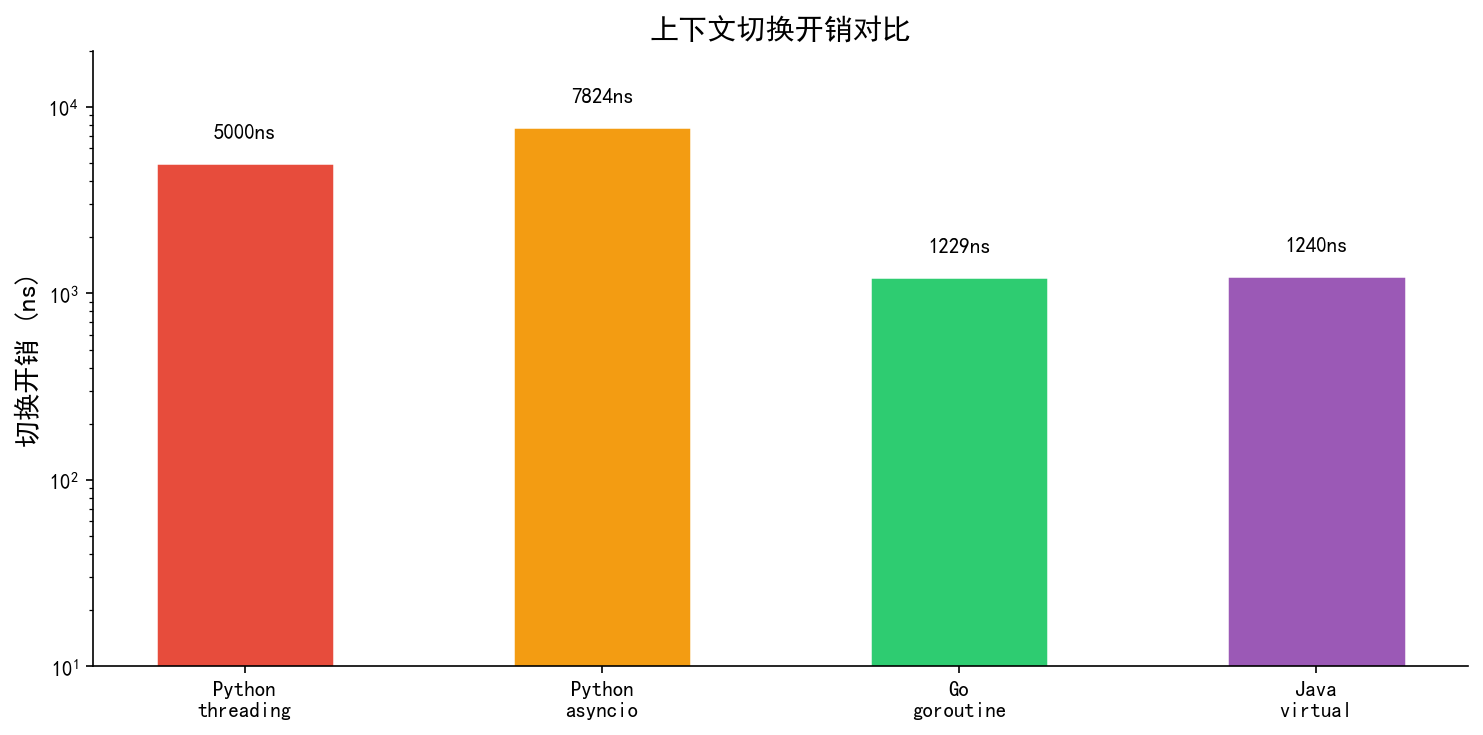
\includegraphics[width=\linewidth]{switch_overhead.png}
    \caption{切换/轻量任务开销量级}
  \end{subfigure}
  \caption{CPU 密集型和调度开销实验}
  \label{fig:cpu-switch}
\end{figure}

Python 的 threading 与 asyncio 在 CPU 密集型测试中都没有获得真正的多核计算收益，threading 还会额外承担大量线程创建和 GIL 竞争开销；这说明协程并不会减少计算本身的 CPU 成本。Go 和 Java 的 CPU 测试更快，主要原因不是 ``协程让计算变快''，而是运行时可以把任务分配到多核上执行。Java 平台线程池在该测试中略快于虚拟线程，也说明虚拟线程的优势不在短小 CPU 任务，而在大量阻塞等待任务。

切换开销图使用对数坐标展示量级差异，三组微基准的实测量级如下：
\begin{itemize}
  \item Python asyncio：百万次 yield 约为 2.494$\pm$0.144 秒；
  \item Go goroutine：100000 次 channel 交互约为 122$\pm$15 ms；
  \item Java 虚拟线程：100000 个 sleep(0) 任务约为 75$\pm$32 ms。
\end{itemize}
由于不同语言的微基准并不完全等价，这些数字更适合用于判断量级，而不应作为绝对排名。

从实验解释上看，CPU 密集测试与 I/O 密集测试正好形成对照：协程可以把等待时间交还给调度器，却不能消除斐波那契递归本身的指令数。Go 和 Java 在该实验中表现更好，主要是因为运行时和线程池能够使用多核，而不是因为 goroutine 或 virtual thread 改变了算法复杂度。这也是报告和展示中需要反复强调的边界：协程是高并发 I/O 工具，不是通用并行计算工具。

\subsection{Java virtual thread pinning：轻量线程的硬边界}

Java 21 的 virtual thread 让同步风格代码可以承载大量阻塞等待，但 JEP 444 明确指出，虚拟线程在某些场景下不能从 carrier 线程卸载，例如在 \verb|synchronized| 代码块或方法中阻塞，或执行某些 native/foreign 调用时发生阻塞\cite{jep444}。这类现象通常称为 pinning：虚拟线程本身很轻，但承载它的 carrier 被固定住，调度器无法把这个 OS 线程拿去运行其他虚拟线程。

为了验证这个边界，本文构造了 120 个 virtual thread，每个任务 sleep 100 ms，并把 JVM 虚拟线程调度器并行度设为 4。未固定版本直接 sleep；固定版本在每个任务自己的 \verb|synchronized| 块内 sleep，避免锁竞争本身成为瓶颈，主要暴露 ``阻塞期间 carrier 无法卸载'' 的影响。实验结果如表 \ref{tab:pinning} 所示。

\begin{table}[H]
  \centering
  \caption{Java virtual thread pinning 实验结果（120 个任务，3 次重复）}
  \begin{tabularx}{\textwidth}{l l X}
    \toprule
    模式 & 总耗时 & 解释 \\
    \midrule
    virtual thread 普通 sleep & 125$\pm$12 ms & 大量虚拟线程在 sleep 时可从 carrier 卸载 \\
    \texttt{synchronized} 内 sleep & 3237$\pm$5 ms & 阻塞期间 carrier 被固定，占满 4 个调度线程后排队 \\
    \bottomrule
  \end{tabularx}
  \label{tab:pinning}
\end{table}

pinning 版本约慢 25.9 倍。这个数量级与理论预期接近：如果只有 4 个 carrier 能并行承载被固定的阻塞任务，120 个 100 ms sleep 至少需要约 $\lceil 120/4\rceil \times 100\text{ ms}=3000\text{ ms}$，实测 3237 ms 还包含任务创建、调度和计时开销。这个实验的意义不在于否定 virtual thread，而是给出更准确的选型边界：它非常适合大量可被 JVM 接管的阻塞 I/O，但旧代码中长时间持有 \verb|synchronized| 锁、JNI/native 调用或不可中断阻塞 API 时，仍可能退化为 carrier 线程排队。

\subsection{内存使用对比}

\begin{figure}[H]
  \centering
  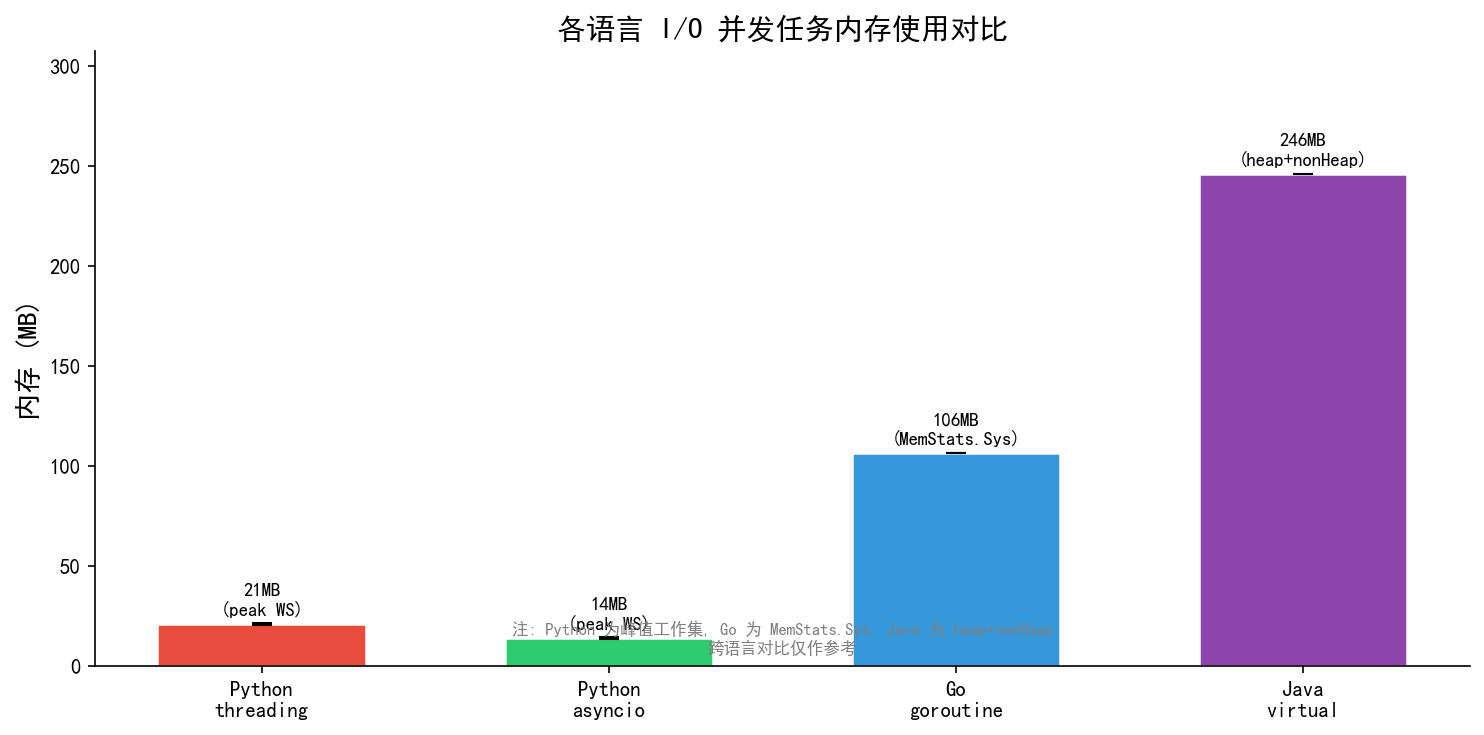
\includegraphics[width=0.70\textwidth]{memory_usage.png}
  \caption{各语言 I/O 并发任务内存使用对比（10K 任务）}
  \label{fig:memory}
\end{figure}

本次实验中，Python 使用采样线程记录 benchmark 期间的进程峰值工作集，Go 使用 \verb|runtime.ReadMemStats| 的 \verb|Sys| 字段，Java 使用 \verb|MemoryMXBean| 的 heap + nonHeap 用量。三种语言使用不同的内存测量方法和运行时模型，因此跨语言对比仅作参考。Python 的内存优势主要来自协程 frame 极小（几十到几百字节）；Go/Java 的较高内存反映了运行时系统本身（调度器、GC、JIT 编译器等）的开销。

\subsection{实验有效性与局限性}

为了避免把实验结果过度解释，本文从三个角度评估有效性。

\begin{itemize}
  \item \textbf{内部有效性}：基础微基准和 TCP echo 在同一台机器上连续运行 5 次，pinning 实验连续运行 3 次，并报告均值和标准差。Java 虚拟线程 I/O 与 TCP echo 的标准差较大，说明 JIT 预热、JVM 初始状态、Windows loopback 与短时间大量连接都会影响结果，因此本文主要解释数量级和机制方向，不把单个耗时当作稳定精确值。
  \item \textbf{构造有效性}：sleep 测试能隔离调度模型差异，衡量 ``等待任务承载能力''；TCP echo 加入真实 socket 生命周期，但仍只覆盖 loopback 上的短连接；pinning 测试用独立锁避免锁竞争，主要观察 synchronized 阻塞对 carrier 的影响。三类实验组合起来，比单纯 sleep 更能说明协程优势和边界，但仍不是完整 Web 服务吞吐测试。
  \item \textbf{外部有效性}：实验只覆盖 Python、Go、Java 三种实现，且运行于 Windows/i9-13900H 本机。Linux epoll、Windows IOCP、不同 JVM 参数、不同 Go/Python 版本、真实网络延迟和服务端框架都可能改变绝对数值；但 ``I/O 等待中协程更省线程资源，CPU 密集不自动变快，阻塞边界会破坏轻量调度'' 这一组结论与主流协程设计文档一致。
\end{itemize}

本次实验存在以下局限性，读者在参考数据时应注意：

\begin{enumerate}
  \item \textbf{I/O 模拟}：\verb|sleep(0.1s)| 只模拟等待，不涉及真实协议栈；本地 TCP echo 覆盖了 socket 生命周期，但仍没有覆盖跨机器网络、HTTP/TLS 或数据库驱动。
  \item \textbf{CPU 测试}：\verb|fib(25)| 用来展示 ``协程不自动加速计算''；Go/Java 的优势来自多核调度，不来自协程语义本身。
  \item \textbf{切换测试}：Python asyncio yield、Go channel、Java sleep(0) 的操作不完全同构，适合看数量级，不适合做精确排名。
  \item \textbf{pinning 测试}：本实验通过限制虚拟线程调度器并行度放大边界效应，便于观察机制；真实系统中的影响取决于锁持有时间、阻塞 API 类型和 carrier 并行度。
  \item \textbf{内存测试}：三种语言使用不同测量方法，跨语言对比仅作参考。
  \item \textbf{未覆盖端到端服务}：没有纳入 HTTP server、数据库连接池、TLS、日志和序列化等真实应用开销，后续可用 FastAPI/Go net/http/Java Loom web server 构造端到端压力测试。
\end{enumerate}

% ============================================================
\section{选型建议与总结}
% ============================================================

\subsection{选型建议}

如果项目瓶颈在 CPU，优先考虑并行计算手段，而不是协程。如果瓶颈在 I/O 且并发量较小，传统线程池已经足够；当并发量达到数千以上时，再考虑协程或虚拟线程。新建高并发后端服务可以优先考虑 Go goroutine；JVM 旧系统希望保留同步代码风格时，Java 21 虚拟线程很有吸引力；Python Web 或爬虫任务适合 asyncio/FastAPI/uvloop，但必须严格避免阻塞调用；系统级高性能服务可以考虑 Rust tokio 或 C++20 协程与 io\_uring/asio 组合。

\begin{table}[H]
  \centering
  \caption{面向工程场景的协程选型建议}
  \begin{tabularx}{\textwidth}{lXX}
    \toprule
    场景 & 推荐方向 & 主要理由与注意事项 \\
    \midrule
    CPU 密集计算 & 多线程/多进程/SIMD/GPU & 协程不能减少计算量，只能改善等待和调度开销。 \\
    新建高并发后端 & Go goroutine & 语言和运行时一体化，GMP、netpoller 与标准库协同成熟。 \\
    JVM 旧系统迁移 & Java 21 虚拟线程 & 同步代码改造成本低，但需关注 \texttt{synchronized}、JNI 和 pinning。 \\
    Python Web/爬虫 & asyncio/FastAPI/uvloop & 上手快，生态成熟；必须避免同步阻塞调用进入事件循环。 \\
    系统级低延迟服务 & Rust tokio 或 C++20 + asio/io\_uring & 控制力强、开销低，但学习和工程复杂度更高。 \\
    \bottomrule
  \end{tabularx}
  \label{tab:selection}
\end{table}

实际选型时可以按三个问题快速判断：第一，瓶颈是否真的在 I/O 等待；第二，现有阻塞 API 能否被运行时接管或替换为异步 API；第三，错误、取消和超时能否被结构化管理。如果这三个问题都能得到肯定回答，协程通常会比传统线程池更适合高并发 I/O；反之，盲目引入 async/await 可能只会增加函数颜色和调试复杂度。

\subsection{总结}

协程的本质不是 ``神奇的快速线程''，而是把等待态任务从昂贵的内核线程中解放出来，用编译器状态机、用户态调度器和操作系统 I/O 多路复用共同支撑高并发。它让程序员可以用近似同步的代码表达异步控制流，是云时代服务端编程的重要抽象。

从技术趋势看，协程正在朝两个方向发展：一类是 C++20/Rust/Python/C\# 代表的无栈 async/await，强调精细控制和低内存；另一类是 Go goroutine 与 Java 21 虚拟线程代表的有栈轻量线程，强调普通同步代码的可扩展性。面对具体工程问题时，最关键的判断不是 ``哪种协程更先进''，而是瓶颈是否在 I/O、阻塞调用能否被运行时接管、错误和取消能否被结构化管理。

% ============================================================
\section{AI 使用说明}
% ============================================================

按照作业要求，本次调研和材料制作中使用 AI 的方式如下：

\begin{enumerate}
  \item 使用 AI 辅助梳理 ``并发演进--协程原理--语言对比--实验验证--选型建议'' 的讲述结构，再人工调整顺序和重点。
  \item 使用 AI 生成和校对部分示意图、表格和代码片段的表达，但实验代码在本机运行后用真实数据替换。
  \item 使用 AI 帮助检查术语一致性，例如有栈/无栈协程、函数颜色、GMP 调度器、virtual thread pinning 等。
  \item 对关键版本号、JEP/PEP、语言特性和运行时机制回查官方文档或源代码说明，避免把 AI 输出直接当作事实。
  \item 最终 Slides 与报告文字均围绕本人实验和理解重新组织，避免大段复制资料原文。
\end{enumerate}

\newpage
\bibliographystyle{plain}
\bibliography{references}

\end{document}
